%%
%% This is file `sample-sigplan.tex',
%% generated with the docstrip utility.
%%
%% The original source files were:
%%
%% samples.dtx  (with options: `sigplan')
%% 
%% IMPORTANT NOTICE:
%% 
%% For the copyright see the source file.
%% 
%% Any modified versions of this file must be renamed
%% with new filenames distinct from sample-sigplan.tex.
%% 
%% For distribution of the original source see the terms
%% for copying and modification in the file samples.dtx.
%% 
%% This generated file may be distributed as long as the
%% original source files, as listed above, are part of the
%% same distribution. (The sources need not necessarily be
%% in the same archive or directory.)
%%
%% The first command in your LaTeX source must be the \documentclass command.
\documentclass[sigplan,screen,nonacm]{acmart}
\usepackage{color}
\usepackage[colorinlistoftodos]{todonotes}
\usepackage[
    type={CC},
    modifier={by-nc-sa},
    version={4.0},
]{doclicense}
%% NOTE that a single column version is required for 
%% submission and peer review. This can be done by changing
%% the \doucmentclass[...]{acmart} in this template to 
%% \documentclass[manuscript,screen,review]{acmart}
%% 
%% To ensure 100% compatibility, please check the white list of
%% approved LaTeX packages to be used with the Master Article Template at
%% https://www.acm.org/publications/taps/whitelist-of-latex-packages 
%% before creating your document. The white list page provides 
%% information on how to submit additional LaTeX packages for 
%% review and adoption.
%% Fonts used in the template cannot be substituted; margin 
%% adjustments are not allowed.
%%
%% \BibTeX command to typeset BibTeX logo in the docs
\AtBeginDocument{%
  \providecommand\BibTeX{{%
    \normalfont B\kern-0.5em{\scshape i\kern-0.25em b}\kern-0.8em\TeX}}}


%%
%% end of the preamble, start of the body of the document source.
\begin{document}

%%
%% The "title" command has an optional parameter,
%% allowing the author to define a "short title" to be used in page headers.
\title{A Summary of Multipath TCP, Performance Metrics, and Packet Scheduling Methods}

%%
%% The "author" command and its associated commands are used to define
%% the authors and their affiliations.
%% Of note is the shared affiliation of the first two authors, and the
%% "authornote" and "authornotemark" commands
%% used to denote shared contribution to the research.
\author{Cole N. Maxwell}
\email{maxwe206@morris.umn.edu}
\affiliation{%
  \institution{Division of Science and Mathematics 
	\\
        University of Minnesota, Morris
	}
  \city{Morris}
  \state{Minnesota}
  \country{USA}
  \postcode{56267}
}

%%
%% By default, the full list of authors will be used in the page
%% headers. Often, this list is too long, and will overlap
%% other information printed in the page headers. This command allows
%% the author to define a more concise list
%% of authors' names for this purpose.
%\renewcommand{\shortauthors}{Trovato and Tobin, et al.}

%%
%% The abstract is a short summary of the work to be presented in the
%% article.
\begin{abstract}
As modern internet communications networks have developed, multiple transmission vectors have become
available to devices on these complex networks. Today many devices contain hardware to transmit data 
across the internet via cellular, WiFi, and wired connections.

\end{abstract}

\doclicenseThis

%%
%% Keywords. The author(s) should pick words that accurately describe
%% the work being presented. Separate the keywords with commas.



%%
%% This command processes the author and affiliation and title
%% information and builds the first part of the formatted document.
\maketitle

\section{Introduction}
\label{sec:introduction}
Multipath transmission control protocol (MPTCP) is a network protocol that leverages 
the use of multiple transmission methods a devices may have, for example the cellular and WiFi connection of a smart phone, 
to deliver more failure tolerant connections using the device's same Internet Protocol (IP) address. Efficient packet scheduling methods can be challenging in diverse network typologies. Increasing MPTCP's network performance with new packet scheduling methods is an active area of research. Section \ref{sec:background} provides necessary background on
Transmission Control Protocol (TCP), the motivation for the MPTCP extension on top of TCP, and an overview of how MPTCP transmits data. Network metrics used to evaluate network performance are described in section \ref{sec:metrics}. In the New Scheduling Method section there is an explanation of a proposed packet scheduling method for heterogeneous wireless networks. Finally, the results of the proposed packet scheduling method are explained.

\todo[inline, color=orange]{Abstract and Introduction are a work-in-progress}

\section{Background}
\label{sec:background}
The Internet Protocol (IP) is the address system of the Internet and specializes in the function of delivering information from a source device to a target device. Every device connected to the internet is assigned an IP address, which works in a similar fashion to a traditional mailing address used by the Post Office. The data sent by IP is divided into smaller pieces of information called packets. IP attaches additional information to the start and end of each data packet, referred to as the header and footer of a packet. The data that is wrapped by a packet is referred to as a segment. IP works similarly to placing a letter into an envelope, where the letter represents a segment, and a packet represents an envelope. The source and destination address are contained in the packet header much like the return and delivery address of an envelope. IP does not handle packet ordering or error checking and requires another protocol, typically TCP.


\subsection{Transmission Control Protocol}
\label{sec:tcp}
TCP is responsible for providing reliable data transmission that is error-checked upon delivery and presents that data to an application in the correct order. To provide this reliability, TCP requires a client and server to establish a connection before any data transmission can take place. The server must listen for incoming connection requests from clients, which is referred to as passive open listening. To establish a connection the client, or active opener, and server perform an information exchange called a three-way handshake. “During connection establishment, several options can be exchanged between the client and server regarding the parameters of the connection. The most important exchange in the three-way handshake is the synchronization sequence numbers which are used to fix missing or misordered data.\cite{Stevens:2011} The steps of creating a connection are as follows:

\begin{enumerate}
  \item The client sends a synchronize (SYN) informing the server that the client wants to start communication and with what sequence number it starts segments.
  \item The server responds to the client request with an Acknowledgement (ACK) which signifies the response of the segment it received and a synchronization (SYN) signifies with what sequence number it starts its segments.
  \item The client acknowledges (ACK) the response of the server, and they both establish a reliable connection with which they will start data transfer.
\end{enumerate}

\begin{figure}[H]
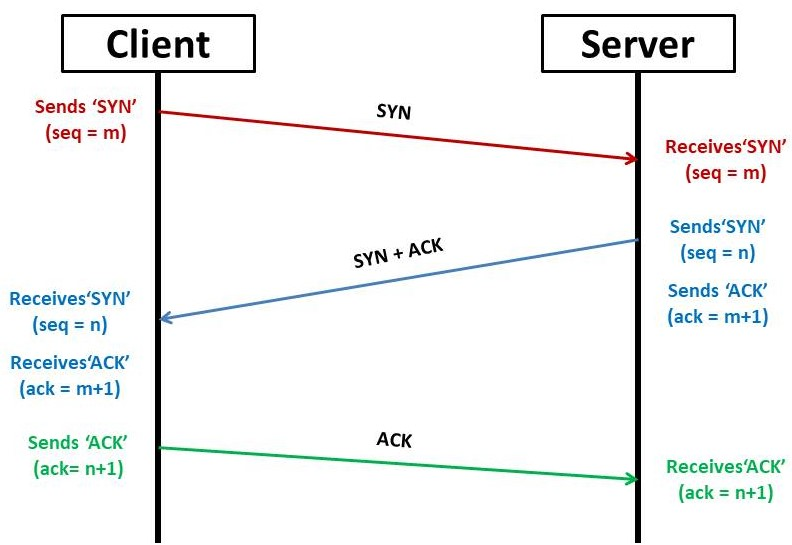
\includegraphics[width=2.5in]{mptcp_paper/assets/tcp-3-way-handshake.jpg}
\caption{An illustration of the TCP three-way handshake}
\label{fig:handshake}
\end{figure}

The sequence number is a counter used by the sender to keep track of every byte sent to a distant end receiver. For example, if a TCP packet contains 1500 bytes of data, the sequence number will be increased by 1500 after the packet is transmitted. In the event that the receiver only receives 1000 bytes, it increases an acknowledgment number by 1000 when it sends out a packet in response. The difference between the sequence and acknowledgment numbers represents the amount of unacknowledged data to the sender. To ensure the receiver has all the data transmitted by the sender, the sender will re-transmit the data until the sequence and acknowledgment numbers are equal. 

While TCP provides reliable data transport, it was originally designed in the early 1970s. During this era, it was extremely uncommon for devices with network interfaces to have multiple mechanisms to deliver packets across a network. In today’s modern networks it is common for devices like smartphones to have cellular and WiFi connections simultaneously. The original TCP design does not allow devices to leverage multiple connections, called subflows, because the connection is bound to the IP addresses of each party's network interface. \cite{MPTCPoverview:2012} Consider the case where a smartphone user is connected to a streaming music service via a WiFi connection. The TCP connection is bound to the IP address assigned to the WiFi interface of the smartphone. If the smartphone is moved from the home to a vehicle, losing WiFi connectivity, the connection will be interrupted. In order to continue the music stream, a new TCP connection must be established using the smartphone’s cellular network connection which is assigned a different IP address. This can result in service interruptions that pause the streaming music while establishing the new TCP connection. Network overhead is also increased when TCP connections need to be reestablished, putting an added burden on service providers.

\subsection{The MPTCP Extension}
\label{sec:mptcp}

To effectively use multiple network connections, the Internet Engineering Task Force (IETF) formally proposed the Multipath TCP extension of TCP in request for comment (RFC) 6824 in January of 2013. The standard was revised in 2020 in RFC 8684. Along with the specification, the RFC details two key features of MPTCP; it is compatible with the existing TCP standard, and MPTCP can operate over the same Internet infrastructure as TCP \cite{MPTCPoverview:2012}. MPTCP establishes a connection using the same three-way handshake described in section \ref{sec:tcp}. However, there are additional options exchanged:

\begin{enumerate}
  \item The client sends a SYN with the MP\_CAPABLE option which indicates the client is capable of using MPTCP. The option contains a token generated by the client, which will be used to identify the MPTCP session.
  \item The server responds with SYN-ACK which contains the MP\_CAPABLE option indicating the server is also capable of MPTCP and also returns a token generated by the server.
  \item The client sends an ACK and the first subflow is established. Data can now be transmitted on the first subflow
\end{enumerate}

Notice that an MPTCP connection must be initialized on a single network interface. In the event that a server does not support MPTCP, the client and server can still use a standard TCP connection upon completion of the handshake, but will not be able to add additional subflows. If the establishment of an MPTCP connection is successful, additional subflows can now be added to the connection. The same three-way handshake described above is performed on the client’s second network interface. The client SYN uses the same client token to ensure that the new subflow is associated with the existing MPTCP connection. This process can be repeated for each network interface.

Multipath TCP can improve network reliability but presents new challenges. The network performance of subflows in an MPTCP connection relies on the condition of its path to the destination. The path condition is determined by link state metrics, such as packet loss rate, queue delay, and throughput capacity. To deal with diverse and changing network conditions across many paths, a scheduler has to select the best available subflow to send each packet. The concept of best subflow depends on the scheduler. Therefore the decision of a packet scheduler plays a key role in MPTCP performance \cite{PacketSchedulingServe:2018}. The diverse situations that can arise in complex networks can cause certain types of scheduling methods to perform well in one scenario and poorly in another. Research into optimal subflow packet scheduling is ongoing.


\section{Performance Metrics}
\label{sec:metrics}
Talks about network performance metrics...

\section{Results}

Talks about results of method...


%%
%% The acknowledgments section is defined using the "acks" environment
%% (and NOT an unnumbered section). This ensures the proper
%% identification of the section in the article metadata, and the
%% consistent spelling of the heading.
\begin{acks}
This is where you thank those who helped you better understand the material 
and gave you helpful feedback on the paper, usually including your adviser. 
This is not a place to thank your family, your significant other or your brest friend, 
or anyone else  for moral support or yummy cookies. 
\end{acks}

%%
%% The next two lines define the bibliography style to be used, and
%% the bibliography file.
\bibliographystyle{ACM-Reference-Format}
\bibliography{mptcp_paper}


\end{document}
\endinput
%%
%% End of file `sample-sigplan.tex'.